%
\documentclass[
  notoc % Suppress Tufte style table of contents.
]{tufte-book}

% Required Tufte packages.
\usepackage{changepage} % or changepage
\usepackage{fancyhdr}
\usepackage{fontenc}
\usepackage{geometry}
\usepackage{hyperref}
\usepackage{natbib}
\usepackage{bibentry}
\usepackage{optparams}
\usepackage{paralist}
\usepackage{placeins}
\usepackage{ragged2e}
\usepackage{setspace}
\usepackage{textcase}
\usepackage{textcomp}
\usepackage{titlesec}
\usepackage{titletoc}
\usepackage{xcolor}
\usepackage{xifthen}

\geometry{paperheight=10in,paperwidth=7in,marginparwidth=30mm,marginparsep=2mm,bindingoffset=10mm,top=10mm,inner=8mm,outer=8mm,bottom=16mm,includehead,includemp}

% Tufte vs. Pandoc workaround.
% Issue: https://github.com/Tufte-LaTeX/tufte-latex/issues/64.
\renewcommand\allcapsspacing[1]{{\addfontfeature{LetterSpace=15}#1}}
\renewcommand\smallcapsspacing[1]{{\addfontfeature{LetterSpace=10}#1}}

% \setmainfont{TeX Gyre Pagella}
\usepackage[utf8]{inputenc}
\usepackage[T1]{fontenc}
\setmainfont{texgyrepagella}[
  Extension = .otf,
  UprightFont = *-regular,
  BoldFont = *-bold,
  ItalicFont = *-italic,
  BoldItalicFont = *-bolditalic,
]

\usepackage{fontspec}
\setmonofont{JuliaMono-Medium.ttf}[
    % Do not remove the trailing forward slash.
    Path = /home/runner/.julia/artifacts/45f34ceb7f1b7b67949715de56b123afeaa72e47/juliamono-0.045/,
    Contextuals = Alternate,
    Ligatures = NoCommon
]

\newfontface\JuliaMonoRegular{JuliaMono-Regular.ttf}[
    Path = /home/runner/.julia/artifacts/45f34ceb7f1b7b67949715de56b123afeaa72e47/juliamono-0.045/,
    Contextuals = Alternate,
    Ligatures = NoCommon
]

\newfontface\JuliaMonoBold{JuliaMono-Bold.ttf}[
    Path = /home/runner/.julia/artifacts/45f34ceb7f1b7b67949715de56b123afeaa72e47/juliamono-0.045/,
    Contextuals = Alternate,
    Ligatures = NoCommon
]



\usepackage{graphicx}
\makeatletter
\def\maxwidth{\ifdim\Gin@nat@width>\linewidth\linewidth\else\Gin@nat@width\fi}
\def\maxheight{\ifdim\Gin@nat@height>\textheight\textheight\else\Gin@nat@height\fi}
\makeatother
% Scale images if necessary, so that they will not overflow the page
% margins by default, and it is still possible to overwrite the defaults
% using explicit options in \includegraphics[width, height, ...]{}
\setkeys{Gin}{width=\maxwidth,height=\maxheight,keepaspectratio}
\DeclareRobustCommand{\href}[2]{#2\footnote{\url{#1}}}

\usepackage{float}
\floatplacement{figure}{H}

% Listings Julia syntax definition.
\input{/home/runner/work/Books.jl/Books.jl/defaults/julia_listings.tex}

% Unicode support.
\input{/home/runner/work/Books.jl/Books.jl/defaults/julia_listings_unicode.tex}

% Used by Pandoc.
\providecommand{\tightlist}{%
  \setlength{\itemsep}{0pt}\setlength{\parskip}{0pt}
}
\newcommand{\passthrough}[1]{#1}

\usepackage{longtable}
\usepackage{booktabs}
\usepackage{array}

% Source: Wandmalfarbe/pandoc-latex-template.
\newlength{\cslhangindent}
\setlength{\cslhangindent}{1.5em}
\newlength{\csllabelwidth}
\setlength{\csllabelwidth}{3em}
\newenvironment{CSLReferences}[2] % #1 hanging-ident, #2 entry spacing
 {% don't indent paragraphs
  \setlength{\parindent}{0pt}
  % turn on hanging indent if param 1 is 1
  \ifodd #1 \everypar{\setlength{\hangindent}{\cslhangindent}}\ignorespaces\fi
  % set entry spacing
  \ifnum #2 > 0
  \setlength{\parskip}{#2\baselineskip}
  \fi
 }%
 {}
\usepackage{calc}
\newcommand{\CSLBlock}[1]{#1\hfill\break}
\newcommand{\CSLLeftMargin}[1]{\parbox[t]{\csllabelwidth}{#1}}
\newcommand{\CSLRightInline}[1]{\parbox[t]{\linewidth - \csllabelwidth}{#1}\break}
\newcommand{\CSLIndent}[1]{\hspace{\cslhangindent}#1}

\definecolor{linkblue}{HTML}{117af2}
\usepackage{hyperref}
\hypersetup{
  colorlinks,
  citecolor=linkblue,
  linkcolor=linkblue,
  urlcolor=linkblue,
  linktoc=page, % Avoid Table of Contents being nearly completely blue.
  pdftitle={Books.jl},
  pdfauthor={Rik Huijzer; and contributors},
  pdflang={en-US},
  breaklinks=true,
  pdfcreator={LaTeX via Pandoc}%
}
\urlstyle{same} % disable monospaced font for URLs

\title{Books.jl}
\author{\noindent{Rik Huijzer}\\[3mm] \noindent{and
contributors}\\[3mm] }
\date{}

% Re-enable section numbering which was disabled by tufte.
\setcounter{secnumdepth}{2}

% Fix captions for longtable.
% Thanks to David Carlisle at https://tex.stackexchange.com/a/183344/92217.
\makeatletter
\def\LT@makecaption#1#2#3{%
  \noalign{\smash{\hbox{\kern\textwidth\rlap{\kern\marginparsep
  \parbox[t]{\marginparwidth}{\vspace{12pt}%
\@tufte@caption@font \@tufte@caption@justification \noindent
   #1{#2: }\ignorespaces #3}}}}}}
\makeatother

% Doesn't seem to do anything.
\usepackage{float}
\floatplacement{figure}{H}
\floatplacement{table}{H}

% Reduce large spacing around sections.
\titlespacing*{\chapter}{0pt}{5pt}{20pt}
\titlespacing*{\section}{0pt}{2.5ex plus 1ex minus .2ex}{1.3ex plus .2ex}
\titlespacing*{\subsection}{0pt}{1.75ex plus 1ex minus .2ex}{1.0ex plus.2ex}

\titleformat{\chapter}%
  [hang]% shape
  {\normalfont\huge\itshape}% format applied to label+text
  {\huge\thechapter}% label
  {1em}% horizontal separation between label and title body
  {}% before the title body
  []% after the title body

% Reduce spacing in table of contents.
\usepackage{etoolbox}
\makeatletter
\pretocmd{\chapter}{\addtocontents{toc}{\protect\addvspace{-3\p@}}}{}{}
\pretocmd{\section}{\addtocontents{toc}{\protect\addvspace{-4\p@}}}{}{}
\pretocmd{\subsection}{\addtocontents{toc}{\protect\addvspace{-5\p@}}}{}{}
\makeatother

% Long texts are harder to read than tables.
% Therefore, we can reduce the font size of the table.
\AtBeginEnvironment{longtable}{\footnotesize}

% Some space between paragraphs is necessary because code blocks can output single line paragraphs.
\setlength\parskip{1em plus 0.1em minus 0.2em}

% For justified text.
\usepackage{ragged2e}

% tufte-book disables subsubsections by default.
% Got this definition back via `\show\subsubsection`.

\usepackage{amsfonts}
\usepackage{amssymb}
\usepackage{amsmath}
\usepackage{unicode-math}

% URL line breaks.
\usepackage{xurl}

% Probably doesn't hurt.
\usepackage{marginfix}

\let\cleardoublepage\clearpage

\usepackage{cancel}

\begin{document}

\makeatletter
\thispagestyle{empty}
\vfill
{\Huge\bf
\noindent
\@title
}\\[1in]
{\Large
\noindent
\@author
}
\makeatother

\makeatletter
\newpage
\thispagestyle{empty}
\vfill
{\noindent
\begin{tabular}{l} Rik Huijzer\\ University of Groningen\\ the Netherlands\\ t.h.huijzer@rug.nl\\ \end{tabular}
}
\vfill
{\small
\url{https://huijzer.xyz/Books.jl/}

2022-08-25

Creative Commons Attribution-NonCommercial-ShareAlike 4.0 International
}
\makeatother


% Don't remove this or authors will show up in header of every page.
\frontmatter
\mainmatter

\setcounter{tocdepth}{1}
\tableofcontents

% Justify text.
\justifying

% parindent seems to be set from within another class too.
% it is really not useful here because it will also indent lines directly after
% code blocks. Which most of the times not useful.
\setlength{\parindent}{0pt}

\hypertarget{sec:about}{%
\chapter{About}\label{sec:about}}

Similar to \href{https://bookdown.org}{Bookdown}, this package wraps
around \href{https://pandoc.org/}{Pandoc}. For websites, this package
allows for:

\begin{itemize}
\tightlist
\item
  Building a website spanning multiple pages.
\item
  Live reloading the website to see changes quickly; thanks to Pandoc
  and \href{https://github.com/tlienart/LiveServer.jl}{LiveServer.jl}.
\item
  Cross-references from one web page to a section on another page.
\item
  Embedding dynamic output, while still allowing normal Julia package
  utilities, such as unit testing and live reloading (Revise.jl).
\item
  Showing code blocks as well as output.
\item
  Interacting with code from within the REPL.
\end{itemize}

If you don't need to generate PDFs, then
\href{https://github.com/tlienart/Franklin.jl}{Franklin.jl} is probably
a better choice. To create single pages and PDFs containing code blocks,
see \href{https://github.com/JunoLab/Weave.jl}{Weave.jl}.

One of the main differences with Franklin.jl, Weave.jl and knitr
(Bookdown) is that this package completely decouples the computations
from the building of the output. The benefit of this is that you can
spawn two separate processes, namely the one to serve your webpages:

\begin{lstlisting}[language=Julia]
$ julia --project -e 'using Books; serve()'
Watching ./pandoc/favicon.png
Watching ./src/plots.jl
[...]
 ✓ LiveServer listening on http://localhost:8001/ ...
  (use CTRL+C to shut down)

\end{lstlisting}

and the one where you do the computations for your package:

\begin{lstlisting}
$ julia --project -ie 'using Books'

julia> gen()
[...]
Updating html
\end{lstlisting}

This way, the website remains responsive when the computations are
running. Thanks to LiveServer.jl and Pandoc, updating the page after
changing text or code takes less than a second. Also, because the
\passthrough{\lstinline!serve!} process does relatively few things, it
almost never crashes.

As another benefit, the decoupling allows you to have more flexibility
in when you want to run what code. In combination with Revise.jl, you
can quickly update your code and see the updated output.

Another reason why this package looks different than other packages is
because this package has been aimed at a REPL workflow. Via the REPL,
the package evaluates the code blocks inside
\passthrough{\lstinline!Main!} by default. This provides easy access to
the variables.

Finally, a big difference with this package and other packages is that
you decide yourself what you want to show for a code block. For example,
in R

\begin{lstlisting}
```{r, results='hide'}
print("Hello, world!")
```
\end{lstlisting}

shows the code and not the output. Instead, in Books, you would write

\begin{lstlisting}
```jl
s = """print("Hello, world!")"""
sc(s)
```
\end{lstlisting}

which is displayed as

\begin{lstlisting}[language=Julia]
print("Hello, world!")
\end{lstlisting}

Here, \passthrough{\lstinline!sc!} is one of the convenience methods
exported by Books.jl. Although this approach is more verbose in some
cases, it is also much more flexible. In essence, you can come up with
your own pre- or post-processing logic. For example, lets write

\begin{lstlisting}
```jl
code = """
    df = DataFrame(a=[1, 2], b=[3, 4])
    Options(df, caption="A table.", label=nothing)
    """
repeat(sco(code), 4)
```
\end{lstlisting}

which shows the code and output (\passthrough{\lstinline!sco!}) 4 times:

\begin{lstlisting}[language=Julia]
df = DataFrame(a=[1, 2], b=[3, 4])
Options(df, caption="A table.", label=nothing)
\end{lstlisting}

\begin{longtable}[]{@{}rr@{}}
\caption{A table.}\tabularnewline
\toprule
a & b \\
\midrule
\endfirsthead
\toprule
a & b \\
\midrule
\endhead
1 & 3 \\
2 & 4 \\
\bottomrule
\end{longtable}

\begin{lstlisting}[language=Julia]
df = DataFrame(a=[1, 2], b=[3, 4])
Options(df, caption="A table.", label=nothing)
\end{lstlisting}

\begin{longtable}[]{@{}rr@{}}
\caption{A table.}\tabularnewline
\toprule
a & b \\
\midrule
\endfirsthead
\toprule
a & b \\
\midrule
\endhead
1 & 3 \\
2 & 4 \\
\bottomrule
\end{longtable}

\begin{lstlisting}[language=Julia]
df = DataFrame(a=[1, 2], b=[3, 4])
Options(df, caption="A table.", label=nothing)
\end{lstlisting}

\begin{longtable}[]{@{}rr@{}}
\caption{A table.}\tabularnewline
\toprule
a & b \\
\midrule
\endfirsthead
\toprule
a & b \\
\midrule
\endhead
1 & 3 \\
2 & 4 \\
\bottomrule
\end{longtable}

\begin{lstlisting}[language=Julia]
df = DataFrame(a=[1, 2], b=[3, 4])
Options(df, caption="A table.", label=nothing)
\end{lstlisting}

\begin{longtable}[]{@{}rr@{}}
\caption{A table.}\tabularnewline
\toprule
a & b \\
\midrule
\endfirsthead
\toprule
a & b \\
\midrule
\endhead
1 & 3 \\
2 & 4 \\
\bottomrule
\end{longtable}

\hypertarget{sec:getting-started}{%
\chapter{Getting started}\label{sec:getting-started}}

The easiest way to get started is to use the template repository at
\url{https://github.com/JuliaBooks/BookTemplate}.

From this repository, you can serve your book via:

\begin{lstlisting}[language=Julia]
$ julia --project -e 'using Books; serve()'
Watching ./pandoc/favicon.png
Watching ./src/plots.jl
[...]
 ✓ LiveServer listening on http://localhost:8001/ ...
  (use CTRL+C to shut down)

\end{lstlisting}

To generate all the Julia output (see Section~\ref{sec:embedding-output}
for more information) use

\begin{lstlisting}
$ julia --project -e  'using Books; using MyPackage'

julia> gen(; )
[...]
Updating html
\end{lstlisting}

where \passthrough{\lstinline!MyPackage!} is the name of your package.
This evaluates all the code from the code blocks inside your
\passthrough{\lstinline!Main!} module. The benefit of this is that you
can easy interact with and access variables defined inside code blocks.

To avoid code duplication between projects, this package tries to have
good defaults for many settings. For your project, you can override the
default settings by creating \passthrough{\lstinline!config.toml!} and
\passthrough{\lstinline!metadata.yml!} files. In summary, the
\passthrough{\lstinline!metadata.yml!} file is read by Pandoc while
generating the outputs. This file contains settings for the output
appearance, author and more, see Section~\ref{sec:metadata}. The
\passthrough{\lstinline!config.toml!} file is read by Books.jl before
calling Pandoc, so contains settings which are essentially passed to
Pandoc, see Section~\ref{sec:config}. Still, these defaults can be
overwritten. If you also want to override the templates, then see
Section~\ref{sec:templates}.

To generate the PDF, use

\begin{lstlisting}
julia> pdf()
\end{lstlisting}

\hypertarget{sec:metadata}{%
\section{metadata.yml}\label{sec:metadata}}

The \passthrough{\lstinline!metadata.yml!} file is read by Pandoc.
Settings in this file affect the behaviour of Pandoc and get inserted in
the templates. For more info on templates, see
Section~\ref{sec:templates}. You can override settings by placing a
\passthrough{\lstinline!metadata.yml!} file at the root directory of
your project. For example, the metadata for this project contains:

\begin{lstlisting}[language=Output]
---
title: Books.jl
subtitle: Create books with Julia
author:
  - Rik Huijzer
  - and contributors

# An example additional header include for html.
# Note that the url will be updated by \`Books.fix_links\`.
header-includes:
- |
  \`\`\`{=html}
  <link rel="stylesheet" href="/files/style.css"/>
  \`\`\`
mousetrap: true

#
# PDF only settings.
#
pdf-footer: ""

# For example, to add extra packages.
extra-pdf-header: |
  \usepackage{cancel}

# Avoid adding a blank page before each chapter.
disable-cleardoublepage: true

bibliography: bibliography.bib

titlepage-top: >
  \begin{tabular}{l}
  Rik Huijzer\\
  University of Groningen\\
  the Netherlands\\
  t.h.huijzer@rug.nl\\
  \end{tabular}

titlepage-bottom: >
  \url{https://huijzer.xyz/Books.jl/}
---

\end{lstlisting}

And, the following defaults are set by Books.jl.

\begin{lstlisting}[language=Output]
---
title: My book
subtitle: My book subtitle
author:
  - John Doe

# Licenses; can be empty.
html-license: <a href="http://creativecommons.org/licenses/by-nc-sa/4.0/">CC BY-NC-SA 4.0</a>
tex-license: Creative Commons Attribution-NonCommercial-ShareAlike 4.0 International

pdf-footer: "\\url{https://github.com/johndoe/Book.jl}"

geometry:
  # Defaulting to large pages to be able to show 92 chars in code blocks.
  - paperheight=10in # 25.4 cm.
  - paperwidth=7in # 17.78 cm.
  - marginparwidth=30mm
  - marginparsep=2mm
  - bindingoffset=10mm
  - top=10mm
  - inner=8mm
  - outer=8mm
  - bottom=16mm
  - includehead
  - includemp

# A setting for the PDF. I don't know whether it is important.
lang: en-US

# Uncomment the following to enable a Chinese/Japanese/Korean (CJK) font.
# CJKmainfont: Noto Serif CJK SC

links-as-notes: true

tags: [pandoc, Books.jl, JuliaLang]
number-sections: true

code-block-font-size: \scriptsize

titlepage: true
linkReferences: true
link-citations: true

# These table of contents settings only affect the PDF.
toc: true
tocdepth: 1

# Cross-reference prefixes.
eqnPrefix: Equation
figPrefix: Figure
tblPrefix: Table
secPrefix: Section

# Keyboard shortcuts.
mousetrap: true

header-left: foobar
---

\end{lstlisting}

Note that Pandoc has a great templating system. For example, the
\href{https://github.com/jgm/pandoc}{Pandoc LaTeX template
``default.latex''} contains hundreds of options which can all be set via
``metadata.yml.'' In the template of this project, I tried to get the
basics right and haven't spend hours on making it configurable. However,
if you want to add options to the templates, feel free to open a pull
request. If you want to configure the template completely by yourself,
you can place ``template.tex'' in ``pandoc/'' at the root of your
project\footnote{With LaTeX, be ready for hours of fiddling to get
  things right though. The current LaTeX template is adjusted to work
  with Tectonic, Julia syntax highlighting and the Tufte LaTeX class.}.
This same holds for the HTML and CSS template.

\hypertarget{sec:config}{%
\section{config.toml}\label{sec:config}}

The \passthrough{\lstinline!config.toml!} file is used by Books.jl.
Settings in this file affect how Pandoc is called. In
\passthrough{\lstinline!config.toml!}, you can define multiple projects;
at least define \passthrough{\lstinline!projects.default!}. The settings
of \passthrough{\lstinline!projects.default!} are used when you call
\passthrough{\lstinline!pdf()!} or \passthrough{\lstinline!serve()!}. To
use other settings, for example the settings for
\passthrough{\lstinline!dev!}, use
\passthrough{\lstinline!pdf(project="dev")!} or
\passthrough{\lstinline!serve(project="dev")!}.

Below, the default configuration is shown. When not defining a
\passthrough{\lstinline!config.toml!} file or omitting any of the
settings, such as \passthrough{\lstinline!port!}, these defaults will be
used. You don't have to copy all these defaults, only \emph{override}
the settings that you want to change. The benefit of multiple projects
is, for example, that you can run a \passthrough{\lstinline!dev!}
project locally which contains more information than the
\passthrough{\lstinline!default!} project. One example could be where
you write a paper, book or report and have a page with some notes.

The meaning of \passthrough{\lstinline!contents!} is discussed in
Section~\ref{sec:about_contents}. The
\passthrough{\lstinline!pdf\_filename!} is used by
\passthrough{\lstinline!pdf()!} and the \passthrough{\lstinline!port!}
setting is used by \passthrough{\lstinline!serve()!}. For this
documentation, the following config is used

\begin{lstlisting}[language=Output]
[projects]

  [projects.default]
  contents = [
    "about",
    "getting-started",
    "demo",
    "references",
  ]
  output_filename = "books"

  # Full URL, required for the sitemap and robots.txt.
  online_url = "https://huijzer.xyz"
  online_url_prefix = "/Books.jl"

  # Extra directories to be copied.
  extra_directories = [
    "images",
    "files"
  ]

  port = 8012

  [projects.notes]
  contents = [
    "demo",
    "notes",
    "references"
  ]

  # This project is only used when testing Books.jl.
  [projects.test]
  contents = [
    "test"
  ]

  online_url = "https://example.com"
  online_url_prefix = "/Example.jl"


\end{lstlisting}

Which overrides some settings from the following default settings

\begin{lstlisting}[language=Output]
[projects]

  # Default project, used when calling serve() or pdf().
  [projects.default]
  homepage_contents = "index"

  metadata_path = "metadata.yml"

  contents = [
    "introduction",
    "analysis",
    "references"
  ]

  # Output filename for the PDF.
  output_filename = "analysis"

  # Full URL, required for the sitemap.
  online_url = "https://example.com"

  # Prefix for GitHub or GitLab Pages.
  online_url_prefix = ""

  # Port used by serve().
  port = 8010

  # Extra directories to be copied from the project root into `_build/`.
  extra_directories = []

  # For large books, it can be nice to show some information on the homepage
  # which is only visible to online visitors and hidden from offline users (PDF).
  include_homepage_outside_html = false

  # Syntax highlighting.
  highlight = true

  # Alternative project, used when calling, for example, serve(project="dev").
  [projects.dev]
  homepage_contents = "index"

  metadata_path = "metadata.yml"

  contents = [
    "introduction",
    "analysis",
    "notes",
    "references"
  ]

  output_filename = "analysis-with-notes"

  port = 8011

  extra_directories = []

  include_homepage_outside_html = false

\end{lstlisting}

Here, the \passthrough{\lstinline!extra\_directories!} allows you to
specify directories which need to be moved into
\passthrough{\lstinline!\_build!}, which makes them available for the
local server and online. This is, for instance, useful for images like
Figure~\ref{fig:store}:

\begin{lstlisting}
![Book store.](images/book-store.jpg){#fig:book_store}
\end{lstlisting}

shows as

\begin{figure}
\hypertarget{fig:store}{%
\centering

\includegraphics{images/book-store.jpg}
\caption{Book store.}\label{fig:store}
}
\end{figure}

\hypertarget{sec:about_contents}{%
\subsection{About contents}\label{sec:about_contents}}

The files listed in \passthrough{\lstinline!contents!} are read from the
\passthrough{\lstinline!contents/!} directory and passed to Pandoc in
the order specified by this list. It doesn't matter whether the files
contain headings or at what levels the heading are. Pandoc will just
place the texts behind each other.

This list doesn't mention the homepage for the website. That one is
specified on a per project basis with
\passthrough{\lstinline!homepage\_contents!}, which defaults to
\passthrough{\lstinline!index!}. The homepage typically contains the
link to the generated PDF. Note that the homepage is only added to the
html output and not to pdf or other outputs.

\hypertarget{website-landing-page}{%
\subsection{Website landing page}\label{website-landing-page}}

By default, Books.jl assumes that you will want a separate landing page
for your book when you host it. This page is not added to the generated
outputs, like PDF, so it's a nice place to put links to the generated
outputs. You will need to create a \passthrough{\lstinline!index.md!}
file in the \passthrough{\lstinline!contents!} directory. Then, using an
top-level header from Markdown (e.g.~``\# Title''), give the file a
title. Immediately after the title, you need to write
\passthrough{\lstinline!\{-\}!} to avoid this chapter showing up in your
HTML menu.

Here is an example of how an example \passthrough{\lstinline!index.md!}
file looks like:

\begin{lstlisting}
# My Book's Awesome Title! {-}

Welcome to the landing page for my awesome book!
\end{lstlisting}

\hypertarget{sec:templates}{%
\section{Templates}\label{sec:templates}}

Unlike \passthrough{\lstinline!metadata.yml!} and
\passthrough{\lstinline!config.toml!}, the default templates should be
good for most users. To override these, create one or more of the files
listed in Table~\ref{tbl:templates}.

\hypertarget{tbl:templates}{}
\begin{longtable}[]{@{}lll@{}}
\caption{\label{tbl:templates}Default templates.}\tabularnewline
\toprule
File & Description & Affects \\
\midrule
\endfirsthead
\toprule
File & Description & Affects \\
\midrule
\endhead
\passthrough{\lstinline!pandoc/style.csl!} & citation style & all
outputs \\
\passthrough{\lstinline!pandoc/style.css!} & style sheet & website \\
\passthrough{\lstinline!pandoc/template.html!} & HTML template &
website \\
\passthrough{\lstinline!pandoc/template.tex!} & PDF template & PDF \\
\bottomrule
\end{longtable}

Here, the citation style defaults to APA, because it is the only style
that I could find that correctly supports parenthetical and in-text
citations. For example,

\begin{itemize}
\tightlist
\item
  in-text: \protect\hyperlink{ref-orwell1945animal}{Orwell}
  (\protect\hyperlink{ref-orwell1945animal}{1945})
\item
  parenthetical: (\protect\hyperlink{ref-orwell1945animal}{Orwell,
  1945})
\end{itemize}

For other citation styles from the
\href{https://github.com/citation-style-language/styles}{citation-style-language},
users have to manually specify the author in the in-text citations.

\hypertarget{sec:demo}{%
\chapter{Demo}\label{sec:demo}}

We can refer to a section with the normal
\href{https://lierdakil.github.io/pandoc-crossref/}{pandoc-crossref}
syntax. For example,

\begin{lstlisting}
See @sec:getting-started.
\end{lstlisting}

See Section~\ref{sec:getting-started}.

\begin{lstlisting}
We can refer to citations such as @orwell1945animal and
[@orwell1949nineteen] or to equations such as @eq:example.
\end{lstlisting}

We can refer to citations such as
\protect\hyperlink{ref-orwell1945animal}{Orwell}
(\protect\hyperlink{ref-orwell1945animal}{1945}) and
(\protect\hyperlink{ref-orwell1949nineteen}{Orwell, 1949}) or to
equations such as Equation~\ref{eq:example}.

\begin{lstlisting}
$$ y = \frac{\sin{x}}{\cos{x}} $$ {#eq:example}
\end{lstlisting}

\begin{equation}\protect\hypertarget{eq:example}{}{ y = \frac{\sin{x}}{\cos{x}} }\label{eq:example}\end{equation}

\begin{lstlisting}
Use single dollar symbols for inline math: $x = 3$.
\end{lstlisting}

Use single dollar symbols for inline math: \(x = 3\).

\hypertarget{sec:embedding-output}{%
\section{Embedding output}\label{sec:embedding-output}}

For embedding code, you can use the \passthrough{\lstinline!jl!} inline
code or code block. For example, to show the Julia version, define a
code block like

\begin{lstlisting}
```jl
YourModule.julia_version()
```
\end{lstlisting}

in a Markdown file. Then, in your package, define the method
\passthrough{\lstinline!julia\_version()!}:

\begin{lstlisting}
julia_version() = "This book is built with Julia $VERSION."
\end{lstlisting}

Next, call \passthrough{\lstinline!using Books, MyPackage!} and
\passthrough{\lstinline!gen()!} to run all the defined in the Markdown
files. If you prefer to be less explicit, you can call
\passthrough{\lstinline!gen(; M=YourModule)!} to allow for:

\begin{lstlisting}
```jl
julia_version()
```
\end{lstlisting}

instead of \passthrough{\lstinline!YourModule.julia\_version()!}. When
passing your module \passthrough{\lstinline!M!} as keyword argument,
\passthrough{\lstinline!Books.jl!} will evaluate all code blocks inside
that module.

Alternatively, if you work on a large project and want to only generate
the output for one or more Markdown files in
\passthrough{\lstinline!contents/!}, such as
\passthrough{\lstinline!index.md!}, use

\begin{lstlisting}[language=Julia]
gen("index")
\end{lstlisting}

Calling \passthrough{\lstinline!gen!} will place the text

\begin{lstlisting}[language=Output]
This book is built with Julia 1.8.0.
\end{lstlisting}

at the right path so that it can be included by Pandoc. You can also
embed output inline with single backticks like

\begin{lstlisting}
`jl YourModule.julia_version()`
\end{lstlisting}

or just call Julia's constant \passthrough{\lstinline!VERSION!} directly
from within the Markdown file. For example,

\begin{lstlisting}
This book is built with Julia `jl VERSION`.
\end{lstlisting}

This book is built with Julia 1.8.0.

While doing this, it is expected that you also have the browser open and
a server running, see Section~\ref{sec:getting-started}. That way, the
page is immediately updated when you run \passthrough{\lstinline!gen!}.

Note that it doesn't matter where you define the function
\passthrough{\lstinline!julia\_version!}, as long as it is in your
module. To save yourself some typing, and to allow yourself to get some
coffee while Julia gets up to speed, you can start Julia for your
package with

\begin{lstlisting}
$ julia --project -ie 'using MyPackage'
\end{lstlisting}

which allows you to re-generate all the content by calling

\begin{lstlisting}
julia> gen()
\end{lstlisting}

To run this method automatically when you make a change in your package,
ensure that you loaded
\href{https://github.com/timholy/Revise.jl}{\passthrough{\lstinline!Revise.jl!}}
before loading your package and run

\begin{lstlisting}[language=Julia]
entr(gen, ["contents"], [MyPackage])
\end{lstlisting}

Which will automatically run \passthrough{\lstinline!gen()!} whenever
one of the files in \passthrough{\lstinline!contents/!} changes or any
code in the \passthrough{\lstinline!MyPackage!} module. To only run
\passthrough{\lstinline!gen!} for one file, such as
\passthrough{\lstinline!contents/my\_text.md!}, use:

\begin{lstlisting}[language=Julia]
entr(() -> gen("my_text"), ["contents"], [MyPackage])
\end{lstlisting}

Or, the equivalent helper function exported by
\passthrough{\lstinline!Books.jl!}:

\begin{lstlisting}[language=Julia]
entr_gen("my_text"; M=[MyPackage])
\end{lstlisting}

With this, \passthrough{\lstinline!gen("my\_text")!} will be called
every time something changes in one of the files in the contents folder
or when something changes in \passthrough{\lstinline!YourModule!}. Note
that you can run this while \passthrough{\lstinline!serve!} is running
in another terminal in the background. Then, your Julia code is executed
and the website is automatically updated every time you change something
in \passthrough{\lstinline!content!} or
\passthrough{\lstinline!MyPackage!}. Also note that
\passthrough{\lstinline!gen!} is a drop-in replacement for
\passthrough{\lstinline!entr\_gen!}, so you can always add or remove
\passthrough{\lstinline!entr\_!} to run a block one time or multiple
times.

In the background, \passthrough{\lstinline!gen!} passes the methods
through
\passthrough{\lstinline!convert\_output(expr::String, path, out::T)!}
where \passthrough{\lstinline!T!} can, for example, be a DataFrame or a
plot. To show that a DataFrame is converted to a Markdown table, we
define a method

\begin{lstlisting}[language=Julia]
my_table() = DataFrame(U = [1, 2], V = [:a, :b], W = [3, 4])
\end{lstlisting}

and add its output to the Markdown file with

\begin{lstlisting}
```jl
BooksDocs.my_table()
```
\end{lstlisting}

Then, it will show as

\hypertarget{tbl:my_table}{}
\begin{longtable}[]{@{}rrr@{}}
\caption{\label{tbl:my_table}My table.}\tabularnewline
\toprule
U & V & W \\
\midrule
\endfirsthead
\toprule
U & V & W \\
\midrule
\endhead
1 & a & 3 \\
2 & b & 4 \\
\bottomrule
\end{longtable}

where the caption and the label are inferred from the
\passthrough{\lstinline!path!}. Refer to Table~\ref{tbl:my_table} with

\begin{lstlisting}
@tbl:my_table
\end{lstlisting}

To show multiple objects, pass a \passthrough{\lstinline!Vector!}:

\begin{lstlisting}[language=Julia]
function multiple_df_vector()
    [DataFrame(Z = [3]), DataFrame(U = [4, 5], V = [6, 7])]
end
BooksDocs.multiple_df_vector()
\end{lstlisting}

\begin{longtable}[]{@{}r@{}}
\toprule
Z \\
\midrule
\endhead
3 \\
\bottomrule
\end{longtable}

\begin{longtable}[]{@{}rr@{}}
\toprule
U & V \\
\midrule
\endhead
4 & 6 \\
5 & 7 \\
\bottomrule
\end{longtable}

When you want to control where the various objects are saved, use
\passthrough{\lstinline!Options!}. This way, you can pass a informative
path with plots for which informative captions, cross-reference labels
and image names can be determined.

\begin{lstlisting}[language=Julia]
function multiple_df_example()
    objects = [
        DataFrame(X = [3, 4], Y = [5, 6]),
        DataFrame(U = [7, 8], V = [9, 10])
    ]
    filenames = ["a", "b"]
    Options.(objects, filenames)
end
BooksDocs.multiple_df_example()
\end{lstlisting}

\hypertarget{tbl:a}{}
\begin{longtable}[]{@{}rr@{}}
\caption{\label{tbl:a}A.}\tabularnewline
\toprule
X & Y \\
\midrule
\endfirsthead
\toprule
X & Y \\
\midrule
\endhead
3 & 5 \\
4 & 6 \\
\bottomrule
\end{longtable}

\hypertarget{tbl:b}{}
\begin{longtable}[]{@{}rr@{}}
\caption{\label{tbl:b}B.}\tabularnewline
\toprule
U & V \\
\midrule
\endfirsthead
\toprule
U & V \\
\midrule
\endhead
7 & 9 \\
8 & 10 \\
\bottomrule
\end{longtable}

To define the labels and/or captions manually, see
Section~\ref{sec:labels-captions}. For showing multiple plots, see
Section~\ref{sec:plots}.

Most things can be done via functions. However, defining a struct is not
possible, because \passthrough{\lstinline!@sco!} cannot locate the
struct definition inside the module. Therefore, it is also possible to
pass code and specify that you want to evaluate and show code (sc)
without showing the output:

\begin{lstlisting}
```jl
s = """
    struct Point
        x
        y
    end
    """
sc(s)
```
\end{lstlisting}

which shows as

\begin{lstlisting}[language=Julia]
struct Point
    x
    y
end
\end{lstlisting}

and show code and output (sco). For example,

\begin{lstlisting}
```jl
sco("p = Point(1, 2)")
```
\end{lstlisting}

shows as

\begin{lstlisting}[language=Julia]
p = Point(1, 2)
\end{lstlisting}

\begin{lstlisting}[language=Output]
Point(1, 2)
\end{lstlisting}

Note that this is starting to look a lot like R Markdown where the
syntax would be something like

\begin{lstlisting}
```{r, results='hide'}
x = rnorm(100)
```
\end{lstlisting}

I guess that there is no perfect way here. The benefit of evaluating the
user input directly, as Books.jl is doing, seems to be that it is more
extensible if I'm not mistaken. Possibly, the reasoning is that R
Markdown needs to convert the output directly, whereas Julia's better
type system allows for converting in much later stages, but I'm not
sure.

\begin{quote}
\textbf{Tip}: When using \passthrough{\lstinline!sco!}, the code is
evaluated in the \passthrough{\lstinline!Main!} module. This means that
the objects, such as the \passthrough{\lstinline!Point!} struct defined
above, are available in your REPL after running
\passthrough{\lstinline!gen()!}.
\end{quote}

\hypertarget{sec:labels-captions}{%
\section{Labels and captions}\label{sec:labels-captions}}

To set labels and captions, wrap your object in
\passthrough{\lstinline!Options!}:

\begin{lstlisting}[language=Julia]
function options_example()
    df = DataFrame(A=[1], B=[2], C=[3])
    caption = "My DataFrame."
    label = "foo"
    return Options(df; caption, label)
end
BooksDocs.options_example()
\end{lstlisting}

\hypertarget{tbl:foo}{}
\begin{longtable}[]{@{}rrr@{}}
\caption{\label{tbl:foo}My DataFrame.}\tabularnewline
\toprule
A & B & C \\
\midrule
\endfirsthead
\toprule
A & B & C \\
\midrule
\endhead
1 & 2 & 3 \\
\bottomrule
\end{longtable}

which can be referred to with

\begin{lstlisting}
@tbl:foo
\end{lstlisting}

\begin{quote}
Table~\ref{tbl:foo}
\end{quote}

It is also possible to pass only a caption or a label. This package will
attempt to infer missing information from the
\passthrough{\lstinline!path!}, \passthrough{\lstinline!caption!} or
\passthrough{\lstinline!label!} when possible:

\begin{lstlisting}[language=Output]
julia> Books.caption_label("foo_bar()", missing, missing)
(caption = "Foo bar.", label = "foo_bar")

julia> Books.caption_label("foo_bar()", "My caption.", missing)
(caption = "My caption.", label = "foo_bar")

julia> Books.caption_label("foo_bar()", "My caption.", nothing)
(caption = "My caption.", label = nothing)

julia> Books.caption_label(missing, "My caption.", missing)
(caption = "My caption.", label = nothing)

julia> Books.caption_label(missing, missing, "my_label")
(caption = "My label.", label = "my_label")

julia> Books.caption_label(missing, missing, missing)
(caption = nothing, label = nothing)
\end{lstlisting}

\hypertarget{sec:function_code_blocks}{%
\section{Obtaining function
definitions}\label{sec:function_code_blocks}}

So, instead of passing a string which \passthrough{\lstinline!Books.jl!}
will evaluate, \passthrough{\lstinline!Books.jl!} can also obtain the
code for a method directly. (Thanks to
\passthrough{\lstinline!CodeTracking.@code\_string!}.) For example,
inside our package, we can define the following method:

\begin{lstlisting}[language=Julia]
function my_data()
    DataFrame(A = [1, 2], B = [3, 4], C = [5, 6], D = [7, 8])
end
\end{lstlisting}

To show code and output (sco) for this method, use the
\passthrough{\lstinline!@sco!} macro. This macro is exported by Books,
so ensure that you have \passthrough{\lstinline!using Books!} in your
package.

\begin{lstlisting}
```jl
@sco BooksDocs.my_data()
```
\end{lstlisting}

This gives

\begin{lstlisting}[language=Julia]
function my_data()
    DataFrame(A = [1, 2], B = [3, 4], C = [5, 6], D = [7, 8])
end
BooksDocs.my_data()
\end{lstlisting}

\hypertarget{tbl:my_data}{}
\begin{longtable}[]{@{}rrrr@{}}
\caption{\label{tbl:my_data}My data.}\tabularnewline
\toprule
A & B & C & D \\
\midrule
\endfirsthead
\toprule
A & B & C & D \\
\midrule
\endhead
1 & 3 & 5 & 7 \\
2 & 4 & 6 & 8 \\
\bottomrule
\end{longtable}

To only show the source code, use \passthrough{\lstinline!@sc!}:

\begin{lstlisting}
```jl
@sc BooksDocs.my_data()
```
\end{lstlisting}

resulting in

\begin{lstlisting}[language=Julia]
function my_data()
    DataFrame(A = [1, 2], B = [3, 4], C = [5, 6], D = [7, 8])
end
\end{lstlisting}

To override options for your output, use the
\passthrough{\lstinline!pre!} keyword argument of
\passthrough{\lstinline!@sco!}:

\begin{lstlisting}
```jl
let
    caption = "This caption is set via the pre keyword."
    pre(out) = Options(out; caption)
    @sco pre=pre my_data()
end
```
\end{lstlisting}

which appears to the reader as:

\begin{lstlisting}[language=Julia]
function my_data()
    DataFrame(A = [1, 2], B = [3, 4], C = [5, 6], D = [7, 8])
end
my_data()
\end{lstlisting}

\begin{longtable}[]{@{}rrrr@{}}
\caption{This caption is set via the pre keyword.}\tabularnewline
\toprule
A & B & C & D \\
\midrule
\endfirsthead
\toprule
A & B & C & D \\
\midrule
\endhead
1 & 3 & 5 & 7 \\
2 & 4 & 6 & 8 \\
\bottomrule
\end{longtable}

See \passthrough{\lstinline!?sco!} for more information. Since we're
using methods as code blocks, we can use the code shown in one code
block in another. For example, to determine the mean of column A:

\begin{lstlisting}
```jl
@sco BooksDocs.my_data_mean(my_data())
```
\end{lstlisting}

shows as

\begin{lstlisting}[language=Julia]
function my_data_mean(df::DataFrame)
    Statistics.mean(df.A)
end
BooksDocs.my_data_mean(my_data())
\end{lstlisting}

1.5

Or, we can show the output inline, namely 1.5, by using

\begin{lstlisting}
`jl BooksDocs.my_data_mean(my_data())`
\end{lstlisting}

It is also possible to show methods with parameters. For example,

\begin{lstlisting}
```jl
@sc BooksDocs.hello("" )
```
\end{lstlisting}

shows

\begin{lstlisting}[language=Julia]
hello(name) = "Hello, $name"
\end{lstlisting}

Now, we can show

\begin{lstlisting}[language=Julia]
BooksDocs.hello("World")
\end{lstlisting}

\begin{lstlisting}[language=Output]

Hello, World

\end{lstlisting}

Here, the \passthrough{\lstinline!M!} can be a bit confusing for
readers. If this is a problem, you can export the method
\passthrough{\lstinline!hello!} to avoid it. If you are really sure, you
can export all symbols in your module with something like
\href{https://discourse.julialang.org/t/exportall/4970/16}{this}.

\hypertarget{sec:plots}{%
\section{Plots}\label{sec:plots}}

For image types from libraries that \passthrough{\lstinline!Books.jl!}
doesn't know about such as plotting types from
\passthrough{\lstinline!Plots.jl!} and
\passthrough{\lstinline!Makie.jl!}, it is required to extend two
methods. First of all, extend \passthrough{\lstinline!Books.is\_image!}
so that it returns true for the figure type of the respective plotting
library. For example for \passthrough{\lstinline!Plots.jl!} set

\begin{lstlisting}
import Books

Books.is_image(plot::Plots.Plot) = true
\end{lstlisting}

and extend \passthrough{\lstinline!Books.svg!} and
\passthrough{\lstinline!Books.png!} too. For example, for
\passthrough{\lstinline!Plots.jl!}:

\begin{lstlisting}[language=Julia]
Books.svg(svg_path::String, p::Plot) = savefig(p, svg_path)
\end{lstlisting}

Adding plots to books is actually a bit tricky, because we want to show
vector graphics (SVG) on the web, but these are not supported (well) by
LaTeX. Therefore, portable network graphics (PNG) images are also
created and passed to LaTeX, so set \passthrough{\lstinline!Books.png!}
too:

\begin{lstlisting}[language=Julia]
Books.png(png_path::String, p::Plot) = savefig(p, png_path)
\end{lstlisting}

Then, plotting works:

\begin{lstlisting}[language=Julia]
function example_plot()
    I = 1:30
    plot(I, I.^2)
end
BooksDocs.example_plot()
\end{lstlisting}

\begin{figure}
\hypertarget{fig:example_plot}{%
\centering
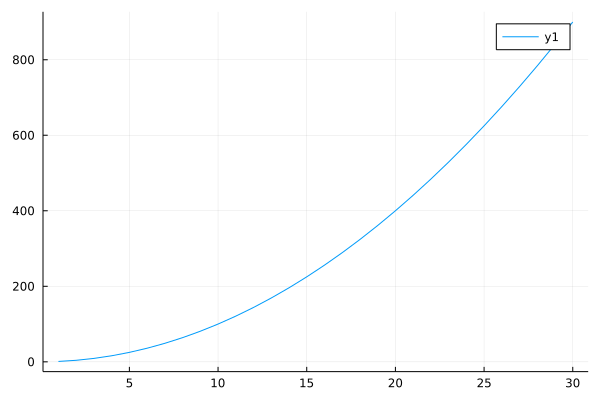
\includegraphics{_build/im/BooksDocs_example_plot_.png}
\caption{Example plot.}\label{fig:example_plot}
}
\end{figure}

For multiple images, use
\passthrough{\lstinline!Options.(objects, paths)!}:

\begin{lstlisting}[language=Julia]
function multiple_example_plots()
    filenames = ["example_plot_$i" for i in 2:3]
    I = 1:30
    objects = [
        plot(I, I.^2),
        scatter(I, I.^3)
    ]
    return Options.(objects, filenames)
end
\end{lstlisting}

Resulting in one \passthrough{\lstinline!Plots.jl!}
(Figure~\ref{fig:example_plot_2}) and one
\passthrough{\lstinline!CairoMakie.jl!}
(Figure~\ref{fig:example_plot_3}) plot:

\begin{figure}
\hypertarget{fig:example_plot_2}{%
\centering
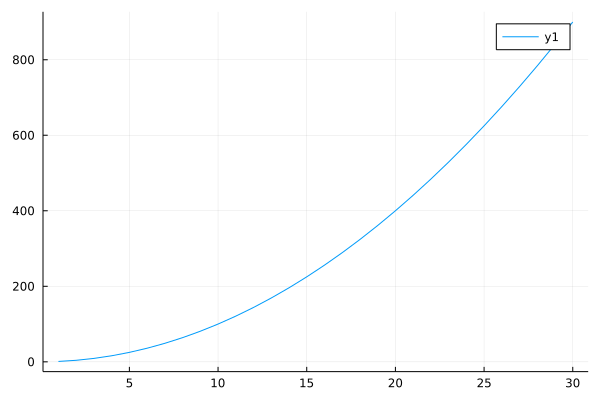
\includegraphics{_build/im/example_plot_2.png}
\caption{Example plot 2.}\label{fig:example_plot_2}
}
\end{figure}

\begin{figure}
\hypertarget{fig:example_plot_3}{%
\centering
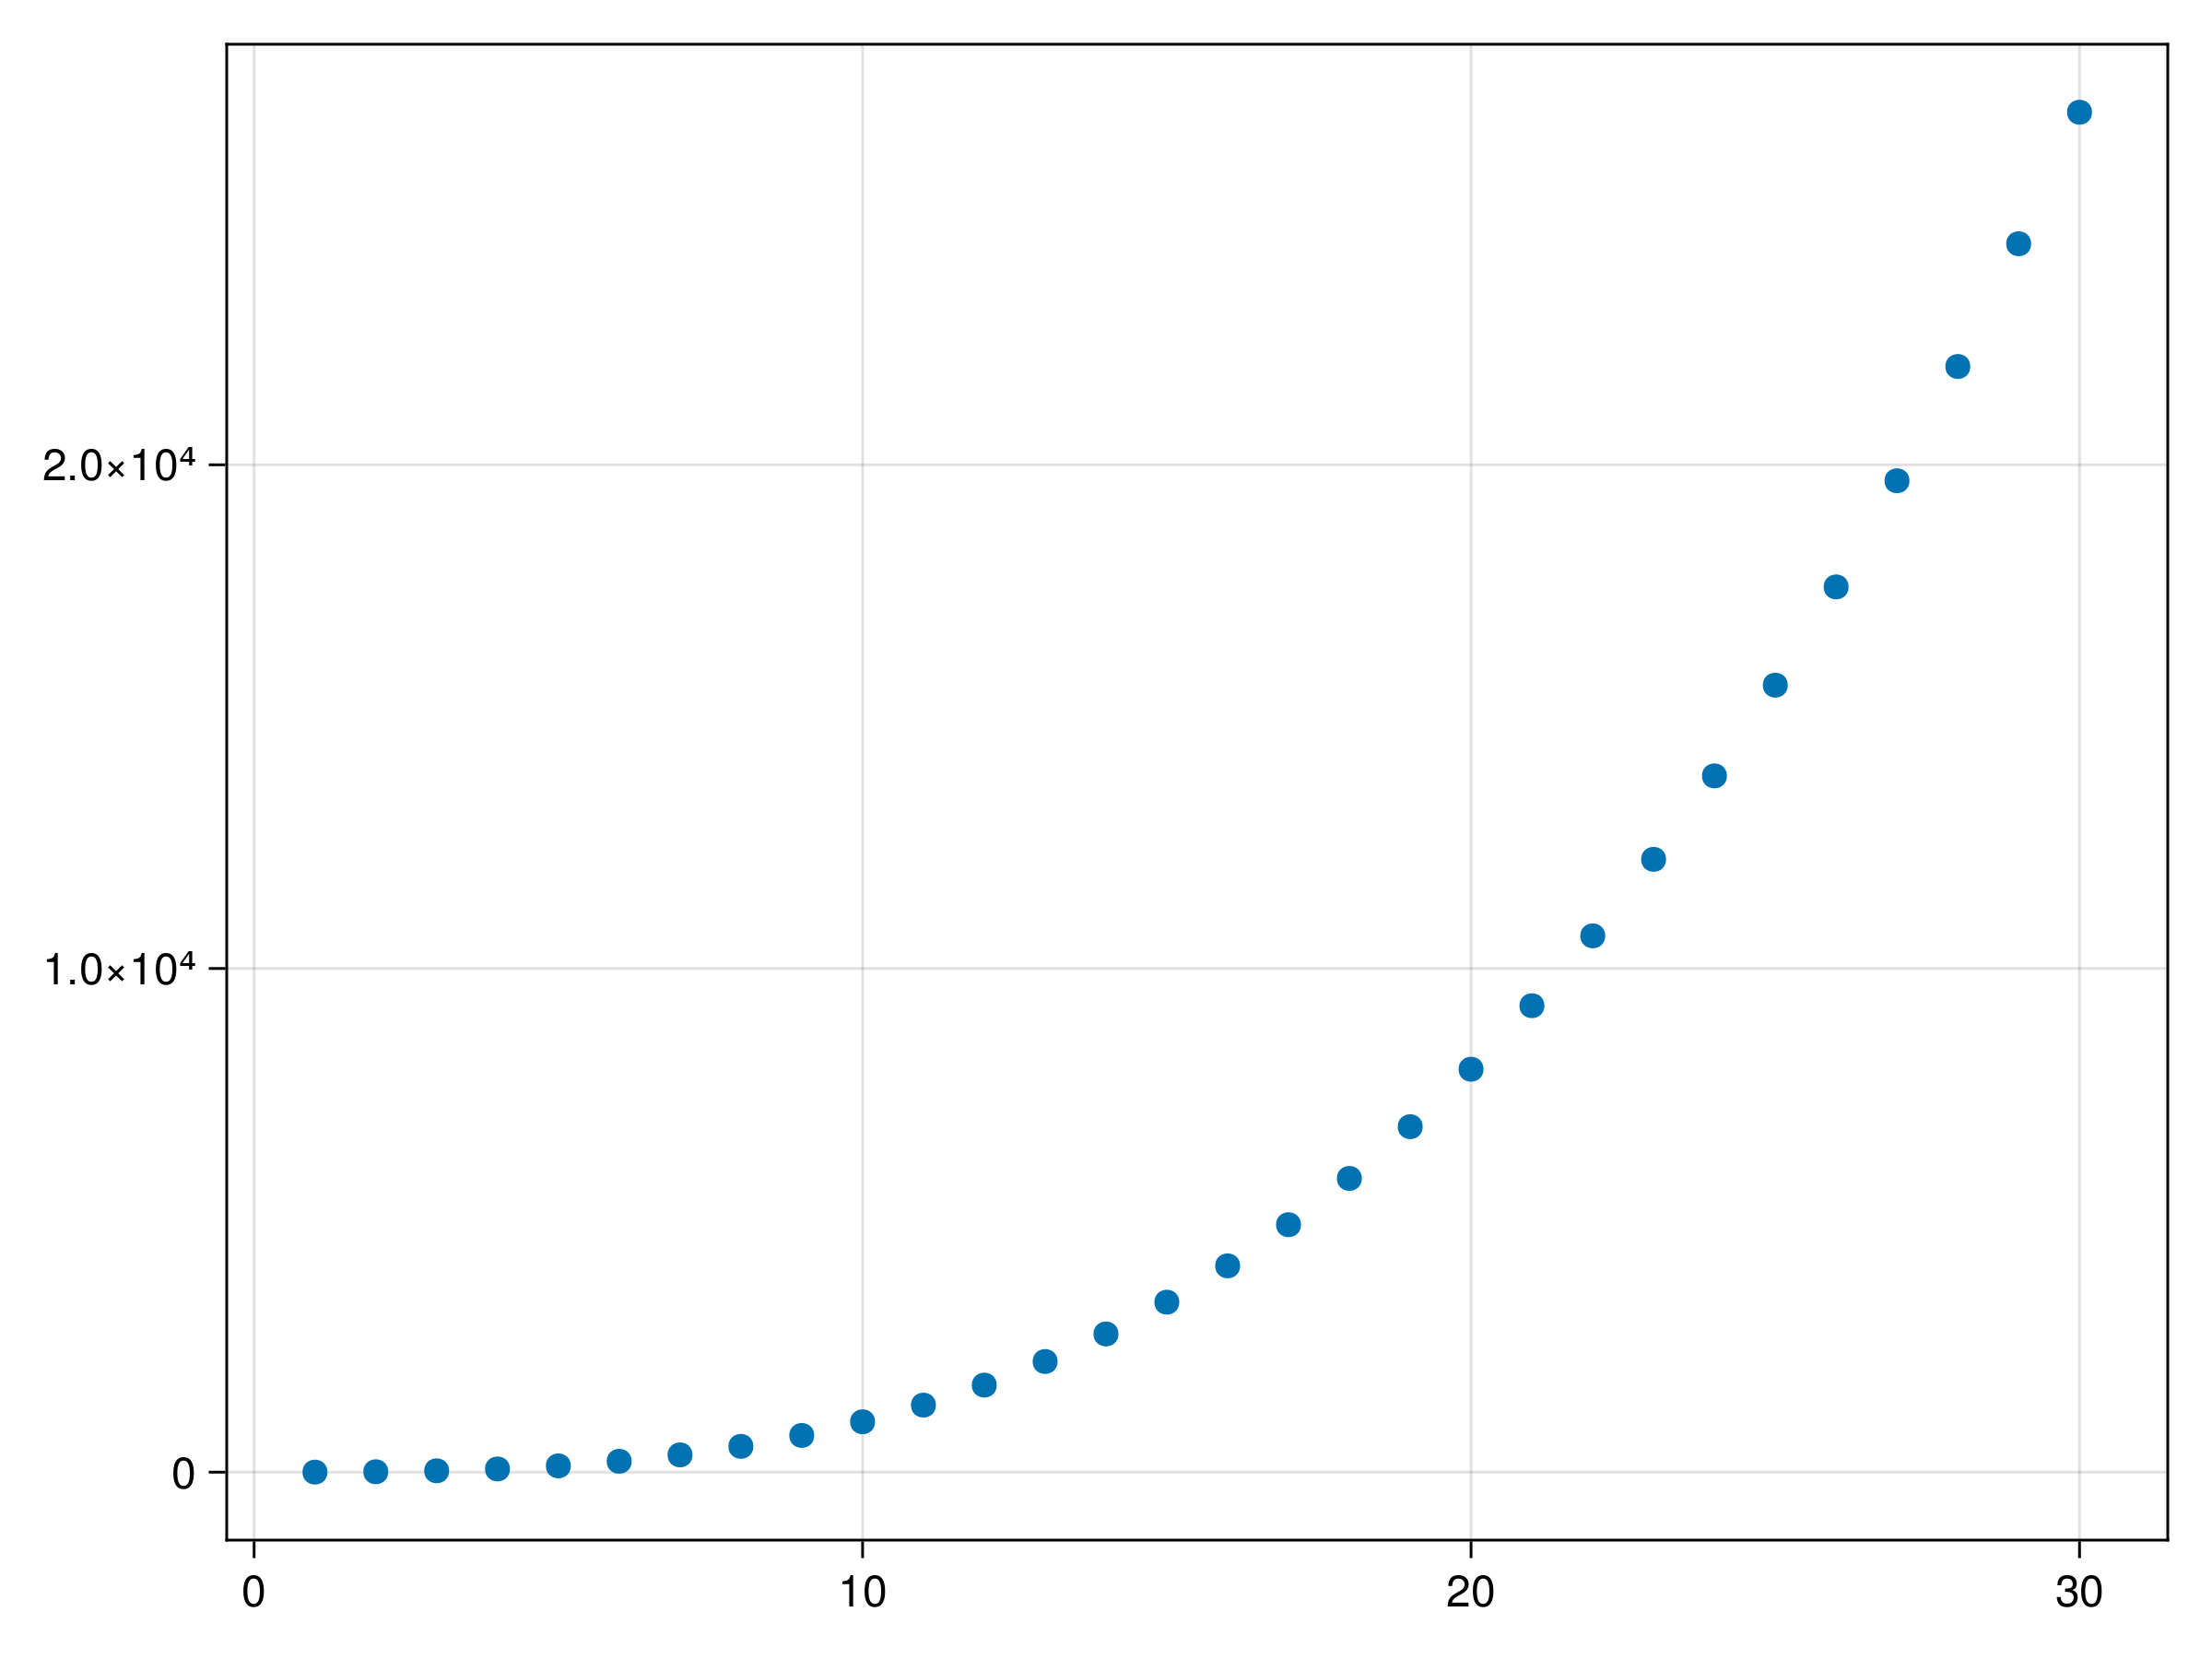
\includegraphics{_build/im/example_plot_3.png}
\caption{Example plot 3.}\label{fig:example_plot_3}
}
\end{figure}

To change the size, change the resolution of the image:

\begin{lstlisting}[language=Julia]
function image_options_plot()
    I = 1:30
    fig = Figure(; resolution=(600, 140))
    ax = Axis(fig[1, 1]; xlabel="x", ylabel="y")
    scatterlines!(ax, I, 3 .* sin.(I))
    return fig
end
BooksDocs.image_options_plot()
\end{lstlisting}

\begin{figure}
\hypertarget{fig:image_options_plot}{%
\centering
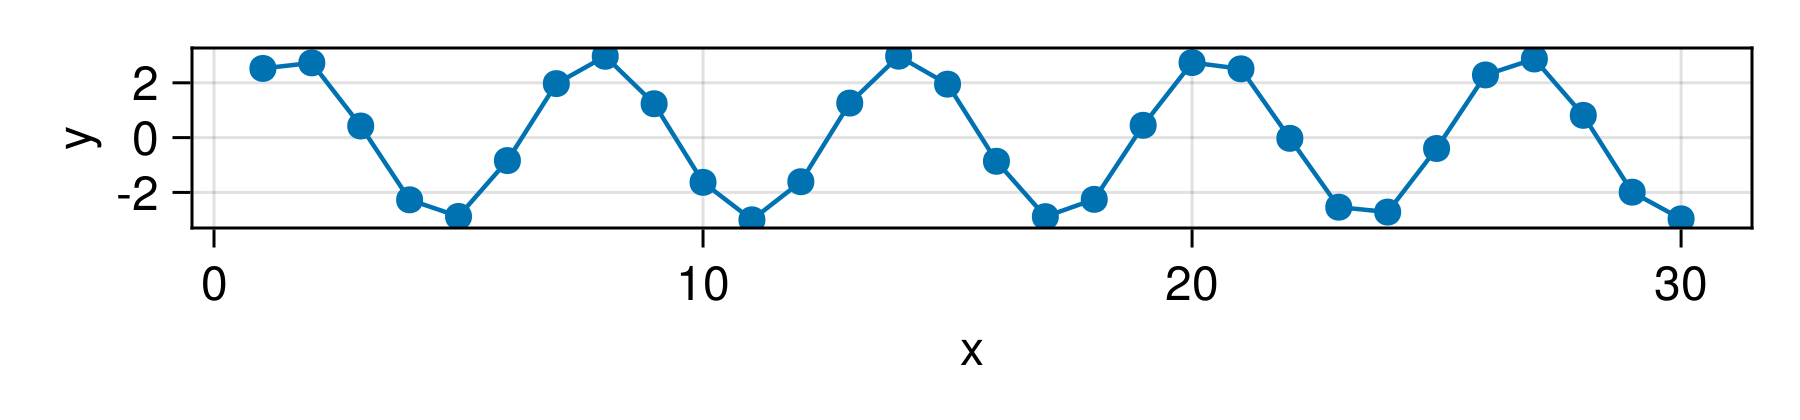
\includegraphics{_build/im/BooksDocs_image_options_plot_.png}
\caption{Image options plot.}\label{fig:image_options_plot}
}
\end{figure}

And, for adjusting the caption, use \passthrough{\lstinline!Options!}:

\begin{lstlisting}[language=Julia]
function combined_options_plot()
    fg = image_options_plot()
    Options(fg; caption="Sine function.")
end
BooksDocs.combined_options_plot()
\end{lstlisting}

\begin{figure}
\centering
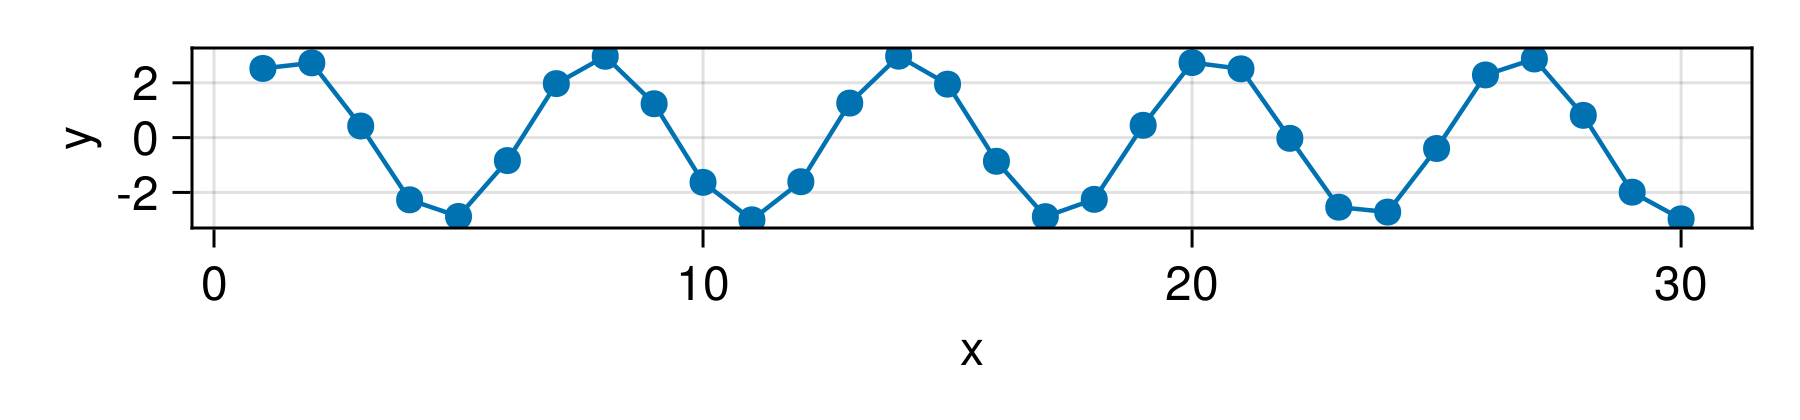
\includegraphics{_build/im/BooksDocs_combined_options_plot_.png}
\caption{Sine function.}
\end{figure}

or the caption can be specified in the Markdown file:

\begin{lstlisting}
```jl
p = BooksDocs.image_options_plot()
Options(p; caption="Label specified in Markdown.")
```
\end{lstlisting}

\begin{figure}
\centering
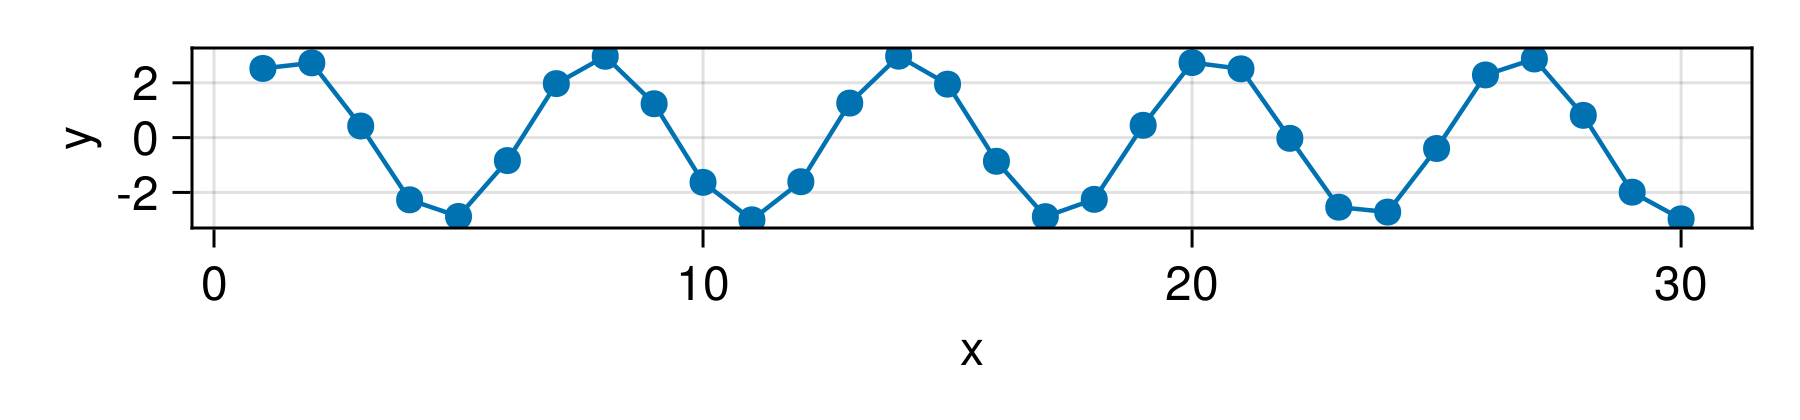
\includegraphics{_build/im/p_BooksDocs_image_options_plot_Options_p_caption_Label_specified_in_Markdo.png}
\caption{Label specified in Markdown.}
\end{figure}

\hfill\break

\begin{lstlisting}[language=Julia]
function plotsjl()
    p = plot(1:10, 1:2:20)
    caption = "An example plot with Plots.jl."
    # Label defaults to `nothing`, which will not create a cross-reference.
    label = missing
    Options(p; caption, label)
end
BooksDocs.plotsjl()
\end{lstlisting}

\begin{figure}
\centering
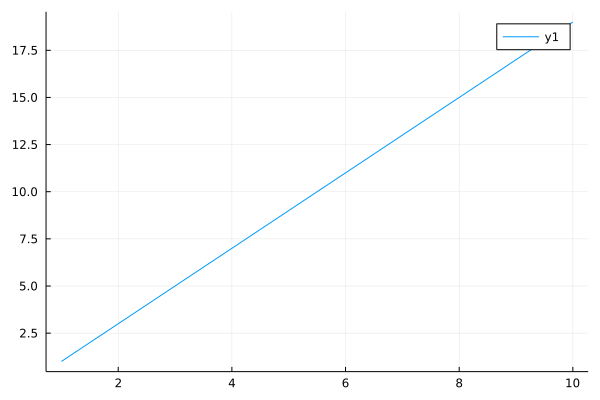
\includegraphics{_build/im/BooksDocs_plotsjl_.png}
\caption{An example plot with Plots.jl.}
\end{figure}

This time, we also pass \passthrough{\lstinline!link\_attributes!} to
Pandoc (Figure~\ref{fig:makie}) to shrink the image width on the page:

\begin{lstlisting}[language=Julia]
function makiejl()
    x = range(0, 10, length=100)
    y = sin.(x)
    p = lines(x, y)
    caption = "An example plot with Makie.jl."
    label = "makie"
    link_attributes = "width=70%"
    Options(p; caption, label, link_attributes)
end
BooksDocs.makiejl()
\end{lstlisting}

\begin{figure}
\hypertarget{fig:makie}{%
\centering
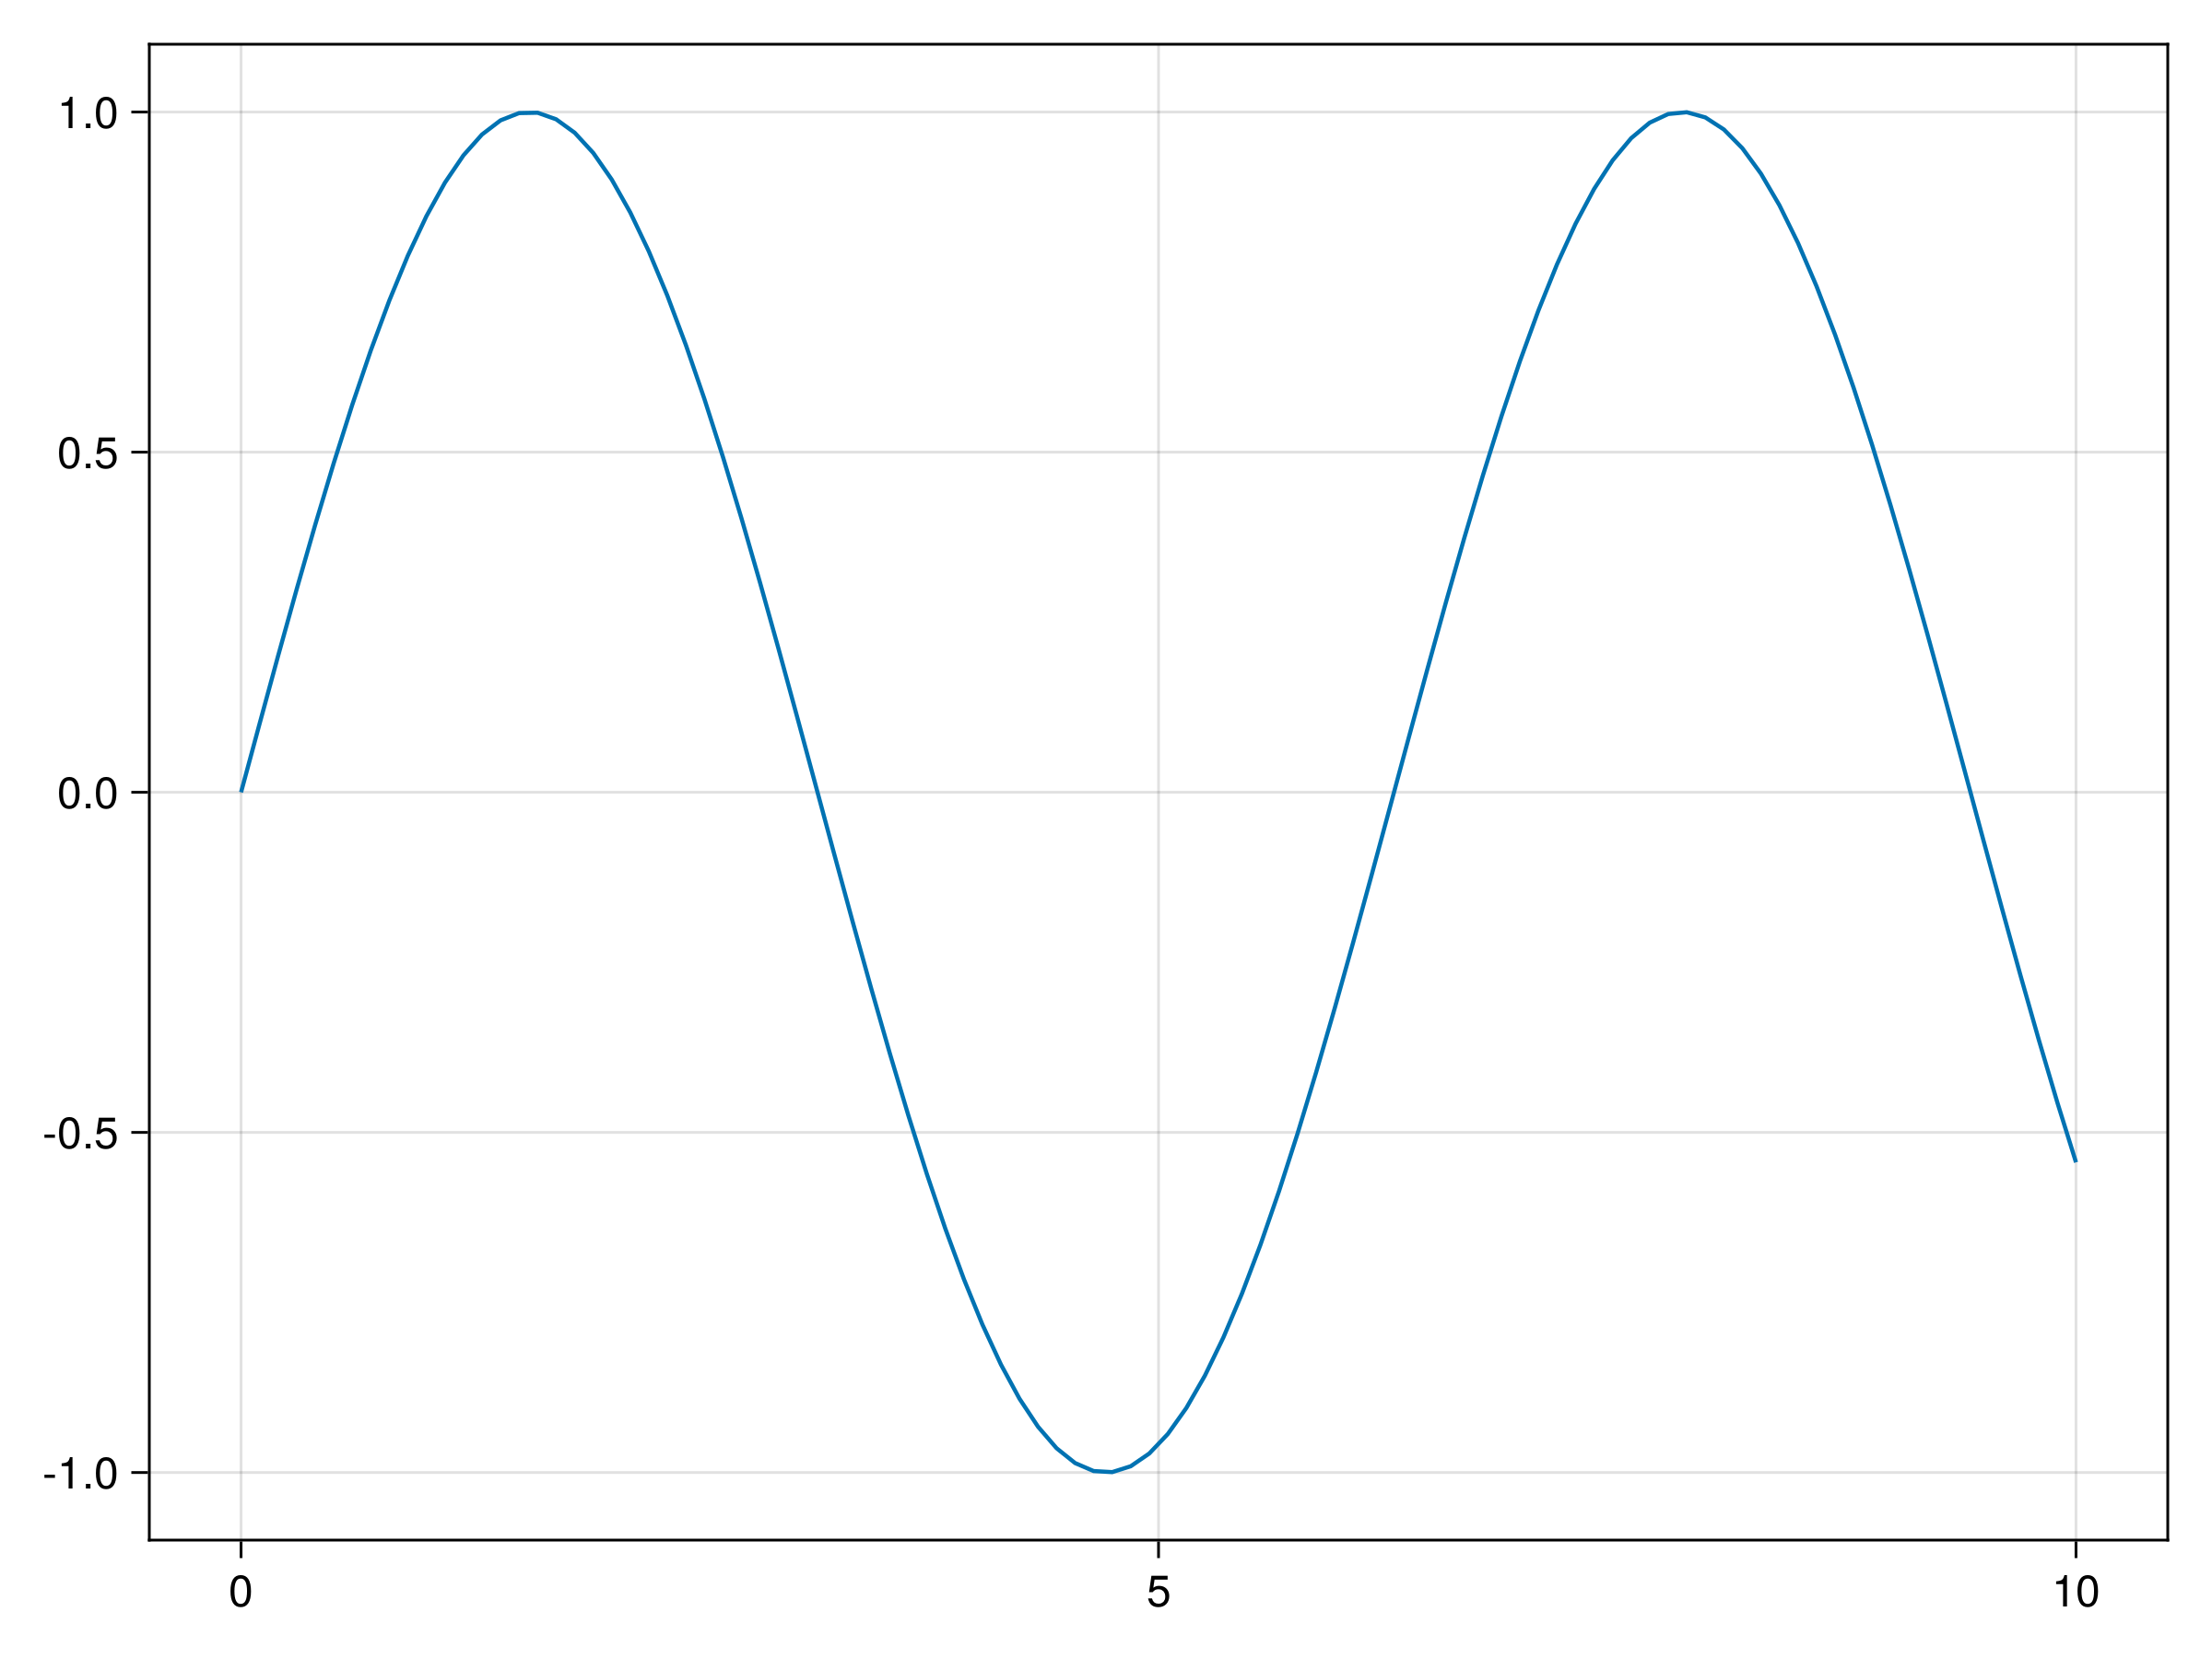
\includegraphics[width=0.7\textwidth,height=\textheight]{_build/im/BooksDocs_makiejl_.png}
\caption{An example plot with Makie.jl.}\label{fig:makie}
}
\end{figure}

\hypertarget{other-notes}{%
\section{Other notes}\label{other-notes}}

\hypertarget{multilingual-books}{%
\subsection{Multilingual books}\label{multilingual-books}}

For an example of a multilingual book setup, say English and Chinese,
see \url{https://juliadatascience.io}.

\hypertarget{footnotes}{%
\subsection{Footnotes}\label{footnotes}}

Footnotes can be added via regular Markdown syntax:

\begin{lstlisting}
Some sentence[^foot].

[^foot]: Footnote text.
\end{lstlisting}

\begin{quote}
Some sentence\footnote{Footnote text.}.
\end{quote}

\hypertarget{show}{%
\subsection{Show}\label{show}}

When your method returns an output type \passthrough{\lstinline!T!}
which is unknown to Books.jl, it will be passed through
\passthrough{\lstinline!show(io::IO, ::MIME"text/plain", object::T)!}.
So, if the package that you're using has defined a new
\passthrough{\lstinline!show!} method, this will be used. For example,
for a grouped DataFrame:

\begin{lstlisting}[language=Julia]
groupby(DataFrame(; A=[1]), :A)
\end{lstlisting}

\begin{lstlisting}[language=Output]
GroupedDataFrame with 1 group based on key: A
Group 1 (1 row): A = 1
 Row │ A
     │ Int64
─────┼───────
   1 │     1
\end{lstlisting}

\hypertarget{note-box}{%
\subsection{Note box}\label{note-box}}

To write note boxes, you can use

\begin{lstlisting}
> **_NOTE:_**  The note content.
\end{lstlisting}

\begin{quote}
\textbf{\emph{NOTE:}} The note content.
\end{quote}

This way is fully supported by Pandoc, so it will be correctly converted
to outputs such as PDF.

\hypertarget{advanced-sco-options}{%
\subsection{\texorpdfstring{Advanced \texttt{sco}
options}{Advanced sco options}}\label{advanced-sco-options}}

To enforce output to be embedded inside a code block, use
\passthrough{\lstinline!scob!}. For example,

\begin{lstlisting}[language=Julia]
scob("
df = DataFrame(A = [1], B = [Date(2018)])
string(df)
")
\end{lstlisting}

\begin{lstlisting}[language=Julia]
df = DataFrame(A = [1], B = [Date(2018)])
string(df)
\end{lstlisting}

\begin{lstlisting}[language=Output]

1×2 DataFrame
 Row │ A      B
     │ Int64  Date
─────┼───────────────────
   1 │     1  2018-01-01

\end{lstlisting}

or, with a string

\begin{lstlisting}[language=Julia]
s = "Hello"
\end{lstlisting}

\begin{lstlisting}[language=Output]

Hello

\end{lstlisting}

Another way to change the output is via the keyword arguments
\passthrough{\lstinline!pre!}, \passthrough{\lstinline!process!} and
\passthrough{\lstinline!post!} for \passthrough{\lstinline!sco!}. The
idea of these arguments is that they allow you to pass a function to
alter the processing that Books.jl does. \passthrough{\lstinline!pre!}
is applied \textbf{before}
\passthrough{\lstinline!Books.convert\_output!},
\passthrough{\lstinline!process!} is applied \textbf{instead} of
\passthrough{\lstinline!Books.convert\_output!} and
\passthrough{\lstinline!post!} is applied \textbf{after}
\passthrough{\lstinline!Books.convert\_output!}. For example, to force
books to convert a DataFrame to a string instead of a Markdown table,
use:

\begin{lstlisting}
```jl
s = "df = DataFrame(A = [1], B = [Date(2018)])"
sco(s; process=string, post=output_block)
```
\end{lstlisting}

which shows the following to the reader:

\begin{lstlisting}[language=Julia]
df = DataFrame(A = [1], B = [Date(2018)])
\end{lstlisting}

\begin{lstlisting}[language=Output]
1×2 DataFrame
 Row │ A      B
     │ Int64  Date
─────┼───────────────────
   1 │     1  2018-01-01
\end{lstlisting}

Without \passthrough{\lstinline!process=string!}, the output would
automatically be converted to a Markdown table by Books.jl and then
wrapped inside a code block, which will cause Pandoc to show the raw
output instead of a table.

\begin{lstlisting}[language=Julia]
df = DataFrame(A = [1], B = [Date(2018)])
\end{lstlisting}

\begin{lstlisting}[language=Output]
|   A |          B |
| ---:| ----------:|
|   1 | 2018-01-01 |

\end{lstlisting}

Without \passthrough{\lstinline!post=output\_block!}, the DataFrame
would be converted to a string, but not wrapped inside a code block so
that Pandoc will treat is as normal Markdown:

\begin{lstlisting}[language=Julia]
df = DataFrame(A = [2], B = [Date(2018)])
\end{lstlisting}

Options(1×2 DataFrame Row │ A B │ Int64 Date ─────┼─────────────────── 1
│ 2 2018-01-01, missing, nothing, nothing, missing)

This also works for \passthrough{\lstinline!@sco!}. For example, for
\passthrough{\lstinline!my\_data!} we can use:

\begin{lstlisting}
```jl
@sco process=string post=output_block my_data()
```
\end{lstlisting}

which will show as:

\begin{lstlisting}[language=Julia]
function my_data()
    DataFrame(A = [1, 2], B = [3, 4], C = [5, 6], D = [7, 8])
end
my_data()
\end{lstlisting}

\begin{lstlisting}[language=Output]
2×4 DataFrame
 Row │ A      B      C      D
     │ Int64  Int64  Int64  Int64
─────┼────────────────────────────
   1 │     1      3      5      7
   2 │     2      4      6      8
\end{lstlisting}

\hypertarget{fonts}{%
\subsection{Fonts}\label{fonts}}

The code blocks default to JuliaMono in HTML and PDF. For the HTML, this
package automatically handles JuliaMono. However, for the PDF, this just
doesn't work out (see, e.g.,
\href{https://github.com/JuliaBooks/Books.jl/pull/257}{257}). To get
JuliaMono to work with the PDF build, install it globally. See the
instructions at the
\href{https://juliamono.netlify.app/download/\#installation}{JuliaMono
site}. On Linux, you can use
\passthrough{\lstinline!Books.install\_extra\_fonts()!}, but beware that
it might override user settings.

Ligatures from JuliaMono are disabled. For example, none of these
symbols are combined into a single glyph.

\begin{lstlisting}
|> => and <=
\end{lstlisting}

\hypertarget{long-lines-in-code-blocks}{%
\subsection{Long lines in code blocks}\label{long-lines-in-code-blocks}}

\begin{lstlisting}
When code or output is getting too long, a horizontal scrollbar is visible on the website to scroll horizontally and a red arrow is visible in the PDF.
\end{lstlisting}

\hypertarget{code-blocks-in-lists}{%
\subsection{Code blocks in lists}\label{code-blocks-in-lists}}

To embed code blocks inside lists, indent by 3 spaces and place an empty
line before and after the code block. For example, this will show as:

\begin{enumerate}
\def\labelenumi{\arabic{enumi}.}
\item
  This is a list item with some code and output:

  \begin{lstlisting}[language=Julia]
  x = 2 + 1
  \end{lstlisting}

  \begin{lstlisting}[language=Output]

  3

  \end{lstlisting}
\item
  And the list continues

  \begin{itemize}
  \item
    with an example on the third level:

    \begin{lstlisting}[language=Julia]
    x = 3 + 1
    \end{lstlisting}

    \begin{lstlisting}[language=Output]

    4

    \end{lstlisting}
  \item
    another third level item
  \item
    and another
  \end{itemize}
\end{enumerate}

\hypertarget{references}{%
\chapter*{References}\label{references}}
\addcontentsline{toc}{chapter}{References}

\hypertarget{refs}{}
\begin{CSLReferences}{1}{0}
\leavevmode\hypertarget{ref-orwell1945animal}{}%
Orwell, G. (1945). \emph{{Animal farm: a fairy story}}. Houghton Mifflin
Harcourt.

\leavevmode\hypertarget{ref-orwell1949nineteen}{}%
Orwell, G. (1949). \emph{{Nineteen eighty-four: a novel}}. Secker \&
Warburg.

\end{CSLReferences}

\backmatter

\end{document}
